\documentclass{beamer}

%
% Choose how your presentation looks.
%
% For more themes, color themes and font themes, see:
% http://deic.uab.es/~iblanes/beamer_gallery/index_by_theme.html
%
\mode<presentation>
{
  \usetheme{default}      % or try Darmstadt, Madrid, Warsaw, ...
  \usecolortheme{default} % or try albatross, beaver, crane, ...
  \usefonttheme{default}  % or try serif, structurebold, ...
  \setbeamertemplate{navigation symbols}{}
  \setbeamertemplate{caption}[numbered]
  \setbeamertemplate{footline}[page number]
  \setbeamercolor{frametitle}{fg=white}
  \setbeamercolor{footline}{fg=black}
} 

\usepackage[english]{babel}
\usepackage[utf8x]{inputenc}
\usepackage{tikz}
\usepackage{listings}
\usepackage{courier}
\usepackage{minted}

\xdefinecolor{darkblue}{rgb}{0.1,0.1,0.7}
\xdefinecolor{dianablue}{rgb}{0.18,0.24,0.31}
\definecolor{commentgreen}{rgb}{0,0.6,0}
\definecolor{stringmauve}{rgb}{0.58,0,0.82}

\lstset{ %
  backgroundcolor=\color{white},      % choose the background color
  basicstyle=\ttfamily\scriptsize,         % size of fonts used for the code
  breaklines=true,                    % automatic line breaking only at whitespace
  captionpos=b,                       % sets the caption-position to bottom
  commentstyle=\color{commentgreen},  % comment style
  escapeinside={\%*}{*)},             % if you want to add LaTeX within your code
  keywordstyle=\color{blue},          % keyword style
  stringstyle=\color{stringmauve},    % string literal style
  showstringspaces=false,
  showlines=true
}

\lstdefinelanguage{scala}{
  morekeywords={abstract,case,catch,class,def,%
    do,else,extends,false,final,finally,%
    for,if,implicit,import,match,mixin,%
    new,null,object,override,package,%
    private,protected,requires,return,sealed,%
    super,this,throw,trait,true,try,%
    type,val,var,while,with,yield},
  otherkeywords={=>,<-,<\%,<:,>:,\#,@},
  sensitive=true,
  morecomment=[l]{//},
  morecomment=[n]{/*}{*/},
  morestring=[b]",
  morestring=[b]',
  morestring=[b]"""
}

\title[2016-10-30-histogrammar-cuda]{Plotting data on GPUs with Histogrammar}
\author{Jim Pivarski}
\institute{Princeton -- DIANA}
\date{September 30, 2016}

\begin{document}

\logo{\pgfputat{\pgfxy(0.11, 8)}{\pgfbox[right,base]{\tikz{\filldraw[fill=dianablue, draw=none] (0 cm, 0 cm) rectangle (50 cm, 1 cm);}}}\pgfputat{\pgfxy(0.11, -0.6)}{\pgfbox[right,base]{\tikz{\filldraw[fill=dianablue, draw=none] (0 cm, 0 cm) rectangle (50 cm, 1 cm);}
\includegraphics[height=0.99 cm]{diana-hep-logo.png}\tikz{\filldraw[fill=dianablue, draw=none] (0 cm, 0 cm) rectangle (4.9 cm, 1 cm);}}}}

\begin{frame}
  \titlepage
\end{frame}

\logo{\pgfputat{\pgfxy(0.11, 8)}{\pgfbox[right,base]{\tikz{\filldraw[fill=dianablue, draw=none] (0 cm, 0 cm) rectangle (50 cm, 1 cm);}
\includegraphics[height=1 cm]{diana-hep-logo.png}}}}

% Uncomment these lines for an automatically generated outline.
%\begin{frame}{Outline}
%  \tableofcontents
%\end{frame}

\begin{frame}{Practical introduction}

\begin{block}{Problem:}
\vspace{0.25 cm}
You're developing a numerical algorithm for GPUs (tracking).

\vspace{0.25 cm}
If you were doing it on a CPU, you could visualize the distribution of any intermediate quantity to debug development.

\vspace{0.25 cm}
But a GPU is like a ship in a bottle: hard to get data in and out; can't use standard tools (ROOT TH1) in {\tt \_\_global\_\_} or {\tt \_\_device\_\_} functions.
\end{block}

\vspace{0.25 cm}
\begin{block}{Solution:}
\vspace{0.25 cm}
Use my library (next page).
\end{block}
\end{frame}

%% \begin{frame}[fragile]{Histogrammar}
%% \vspace{0.35 cm}
%% How to plot an intermediate quantity (call it ``{\tt residual}''):

%% \begin{enumerate}
%% \item Define a histogram or suite of histograms (Python).

%% \begin{minted}{python}
%% h = Bin(100, -5.0, 5.0, "residual")
%% \end{minted}

%% \item Generate CUDA code.

%% \begin{minted}{python}
%% open("histogram.cu", "w").write(h.cuda())
%% \end{minted}

%% \item Allocate histograms in your code (CUDA).

%% \scriptsize
%% \begin{minted}{c++}
%% const int numHists = 1024;
%% Aggregator* hists;
%% cudaMalloc((void**)&hists, numHists * sizeof(Aggregator));
%% initialize<<<1, numThreadsPerBlock>>>(hists, numHists);
%% \end{minted}

%% \normalsize
%% \item Fill them in your {\tt \_\_global\_\_} or {\tt \_\_device\_\_} function.

%% \scriptsize
%% \begin{minted}{c++}
%% __global__
%% void yourFunc(Aggregator* hists, int numHists, ...) {
%%   float residual = ...;
%%   fill(hists, numHists, residual);
%% }
%% \end{minted}
%% \end{enumerate}
%% \end{frame}

%% \begin{frame}[fragile]{Histogrammar}
%% \vspace{0.35 cm}
%% \begin{enumerate}
%%   \setcounter{enumi}{4}

%%   \item When you're done, collapse {\tt numHists} histograms into one histogram and bring it back to the CPU.

%% \scriptsize
%% \begin{minted}{c++}
%% Aggregator* resultGPU;
%% cudaMalloc((void**)&resultGPU, sizeof(Aggregator));
%% extract<<<1, numThreadsPerBlock>>>(hists, numHists, resultGPU);

%% // (or use pinned memory to avoid explicit copy).
%% Aggregator resultCPU;
%% cudaMemcpy(&resultCPU, resultGPU, sizeof(Aggregator),
%%            cudaMemcpyDeviceToHost);
%% \end{minted}

%% \normalsize
%% \item Print out the histogram data.

%% \scriptsize
%% \begin{minted}{c++}
%% toJson(&resultCPU, stdout);   // or a FILE* to "h.json"
%% \end{minted}

%% \normalsize
%% \item Plot it in PyROOT (Python).
%% \begin{minted}{python}
%% h = Factory.fromJson(open("h.json").read())
%% roothist = h.plot.root(name="resid")
%% roothist.Draw()
%% \end{minted}

%% \end{enumerate}
%% \end{frame}

\begin{frame}{What just happened?}
\vspace{0.5 cm}
Generates C structs and fill functions specific to your histogram, making no assumptions about number of threads or blocks.

\vspace{0.2 cm}
Whenever one of your kernels calls {\tt fill}, a thread-local histogram is filled. They may be allocated in global memory (this example) or shared memory (more complex).

\vspace{0.2 cm}
The {\tt extract} kernel recursively adds the thread-local histograms into one final histogram (e.g.\ 1024 histograms in 10 steps).

\vspace{0.3 cm}
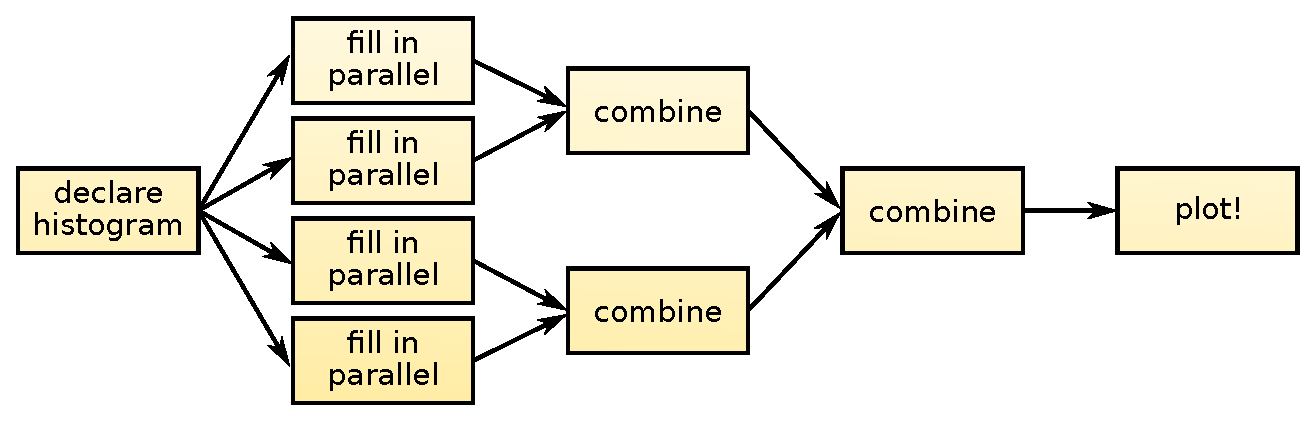
\includegraphics[width=\linewidth]{parallelization.pdf}
\end{frame}

\begin{frame}{Library gets the hard parts right}
\vspace{0.5 cm}
\begin{itemize}\setlength{\itemsep}{0.35 cm}
\item ``Mappers'' (embarrassingly parallel) are easy on GPUs, ``reducers'' are hard because of coordination among threads. Histogram adding is done by library.

\item Number of histograms might be different from number of threads. Generated code uses {\tt \%} and {\tt atomicAdd}.

\vspace{0.2 cm}
(Perhaps that should be optional?)

\item Contiguous in memory for efficient cache usage.

\item Many types of histograms: regular, irregular, N-dimensional, profiles, stacked, efficiency ratio, directories of histograms, etc.

\vspace{0.2 cm}
Actually, a generic grammar for creating new aggregator types.

\item Part of an ecosystem involving much more than GPUs.
\end{itemize}
\end{frame}

\begin{frame}[fragile]{Grammar of histograms}
\begin{center}

\includegraphics[width=0.5\linewidth]{histogrammar-logo.png}
\end{center}
\tiny
\begin{columns}
\column{0.5\linewidth}
\textcolor{darkblue}{\scriptsize Standard histograms:}
\begin{minted}{python}
Bin(num, low, high, fillRule, Count())
\end{minted}

\vspace{0.25 cm}
\textcolor{darkblue}{\scriptsize Two-dimensional histograms:}
\begin{minted}{python}
Bin(xnum, xlow, xhigh, "x",
  Bin(ynum, ylow, yhigh, "y",
    Count()))
\end{minted}

\vspace{0.25 cm}
\textcolor{darkblue}{\scriptsize Profile plots:}
\begin{minted}{python}
Bin(xnum, xlow, xhigh, "y",
  Deviate("y"))

Bin(xnum, xlow, xhigh, "x",
  Bin(ynum, ylow, yhigh, "y",
    Average("z")))
\end{minted}

\vspace{0.25 cm}
\textcolor{darkblue}{\scriptsize Complex trees of aggregations:}
\begin{minted}{python}
Bin(xnum, xlow, xhigh, "x",
  Branch(Minimize("y"),
         Maximize("y"),
         Average("y"),
         Sum("weight"),
         Sum("weight * weight")))
\end{minted}

\column{0.5\linewidth}
\textcolor{darkblue}{\scriptsize Mix and match binning methods:}
\begin{minted}{python}
IrregularlyBin([-2.4, -2.1, -1.5,
    0.0, 1.5, 2.1, 2.4], "eta",
  Bin(314, -3.14, 3.14, "phi",
    Count()))

# don't allocate if zero
SparselyBin(0.01, "eta",
  Bin(314, -3.14, 3.14, "phi",
    Count()))

# bin by strings (bar chart)
Categorize(fillByName,
  Bin(314, -3.14, 3.14, "phi",
    Count()))
\end{minted}

\vspace{0.25 cm}
\textcolor{darkblue}{\scriptsize High-level interface to common patterns:}

\vspace{-0.1 cm}
\begin{minted}{python}
# efficiency plot
Fraction("numHits > 5",
  Bin(numBins, lowEdge, highEdge, "pt"))

# stack of plots with different cuts
Stack([5.0, 10.0, 30.0, 50.0, 100.0], "pt",
  Bin(numBins, lowEdge, highEdge, "numHits"))
\end{minted}
\end{columns}
\end{frame}




\end{document}
